\documentclass[12pt]{article}
\usepackage{graphicx}
\usepackage{setspace}
\usepackage{fancyhdr}
\usepackage{amssymb}
\usepackage{xcolor}
\usepackage{amsmath}
\usepackage{svg}
\usepackage[colorlinks=true, urlcolor=blue]{hyperref}
\usepackage{graphicx}
\usepackage{makecell}
\usepackage{fontawesome5}
\usepackage[a4paper, margin=1in]{geometry}
\pagestyle{fancy}
\lhead{Gravity Anomaly Modeling Using Altimetry Observations}
\rhead{Aliakbar Zarkoob}

\begin{document}
	
	\begin{titlepage}
		\begin{center}
			
			\includegraphics[height=4cm]{University_of_Tehran_Transparent_BW_logo.png} \hfill
			\includegraphics[height=4cm]{Fanni_Alt_BW_Logo.png}
			
			\vspace{1cm}
			
			\Large \textbf{School of Surveying and Geospatial Engineering}\\
			\large {Department of Geodesy and Hydrography}
			
			\vspace{3cm}
			
			\huge \textbf{Gravity Anomaly Modeling Using Altimetry Observations} \\
			\large \href{https://github.com/XIVAliakbarZarkoob/Gravity-Anomaly-Modeling-Using-Altimetry-Observations}{\faGithub}
			
			\vspace{2cm}
			
			\Large \textbf{Author:}\\
			\Large Aliakbar Zarkoob
			
			\vspace{2cm}
			
			\Large \textbf{Professor:}\\
			Dr. Abdolreza Safari
			
			\vfill
			
			\large {Spring 2024}
			
		\end{center}
	\end{titlepage}
	
	
	\section{Introduction}
	
	Gravity anomaly modeling helps improve our understanding of Earth’s internal mass distribution and identify variations in the density of different materials. In this regard, the use of altimetry data as a vast source of elevation information is particularly important, especially in areas where direct access is difficult.
	
	Altimetry, which is primarily conducted via satellites, provides precise information about sea surface height and its variations over time. These data are not only useful for oceanographic studies and monitoring sea level changes but also serve as an auxiliary tool for gravity anomaly modeling. Furthermore, global geoid height models are now available, many of which are calculated using altimetry observations. For example, the EGM2008 model, one of the most comprehensive geoid models, was computed using satellite altimetry data, gravimetry data, as well as seismic data.
	
	In this report, altimetry data are examined for the purpose of gravity anomaly modeling. First, the collection of data and the computation of geoid height from these products are discussed, followed by the modeling of gravity anomalies using these data and a presentation of the results.
	
	\section{Data Collection and Study Area}
	
	In this project, Dynamic Ocean Topography (DOT) and Sea Surface Height (SSH) are used to compute geoid height. The relation between these two parameters and Geoid Height (N), as shown in Figure \ref{fig:relation}, is expressed by Equation \ref{eq:relation}.
	
	\begin{figure}[h!]
		\centering
		\includegraphics[height=7cm]{../Plots/dot_ggos.png}
		\caption{Relation between DOT, SSH, and N.}
		\label{fig:relation}
	\end{figure}
	
	\begin{equation}
		N = SSH - DOT
		\label{eq:relation}
	\end{equation}
	
	For collecting the two mentioned products, the Open Altimeter Database (OpenADB) was used. The study area spans longitudes $326^\circ$ to $360^\circ$ and latitudes $–33^\circ$ to $0^\circ$. The data used are measurements from the SARAL satellite for two months of 2015. The satellite’s coverage for the specified period can be seen in Figure \ref{fig:GT}, and the collected data are shown in Figures \ref{fig:DOT} and \ref{fig:SSH}.
	
	\begin{figure}[h!]
		\centering
		\includegraphics[width=13cm]{../Plots/Screenshot 2024-06-29 183022.png}
		\caption{Ground track of the SARAL satellite for two months of 2015.}
		\label{fig:GT}
	\end{figure}
	
	\begin{figure}[h!]
		\centering
		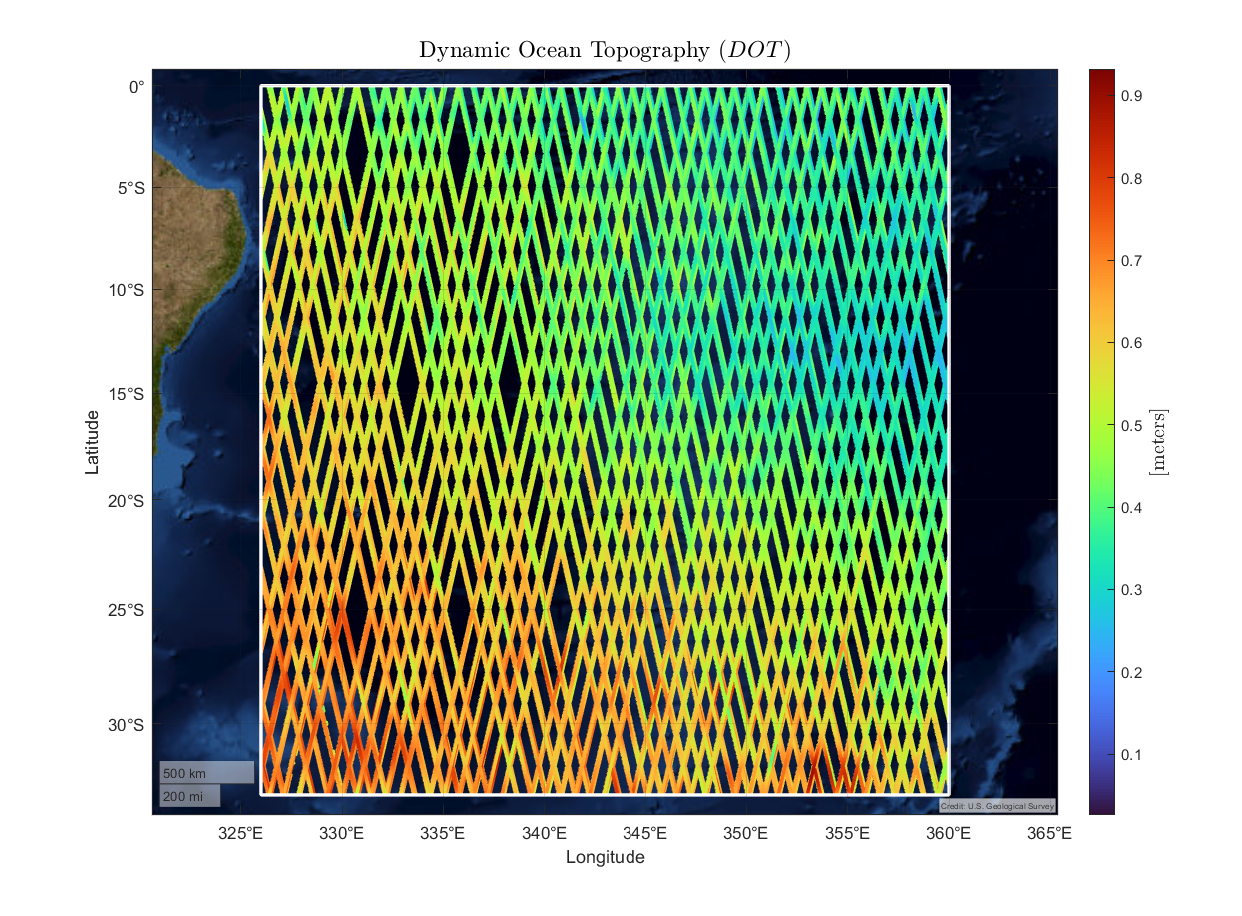
\includegraphics[height=7.5cm]{../Plots/DOT.pdf}
		\caption{DOT values during the specified time period.}
		\label{fig:DOT}
	\end{figure}
	
	\begin{figure}[h!]
		\centering
		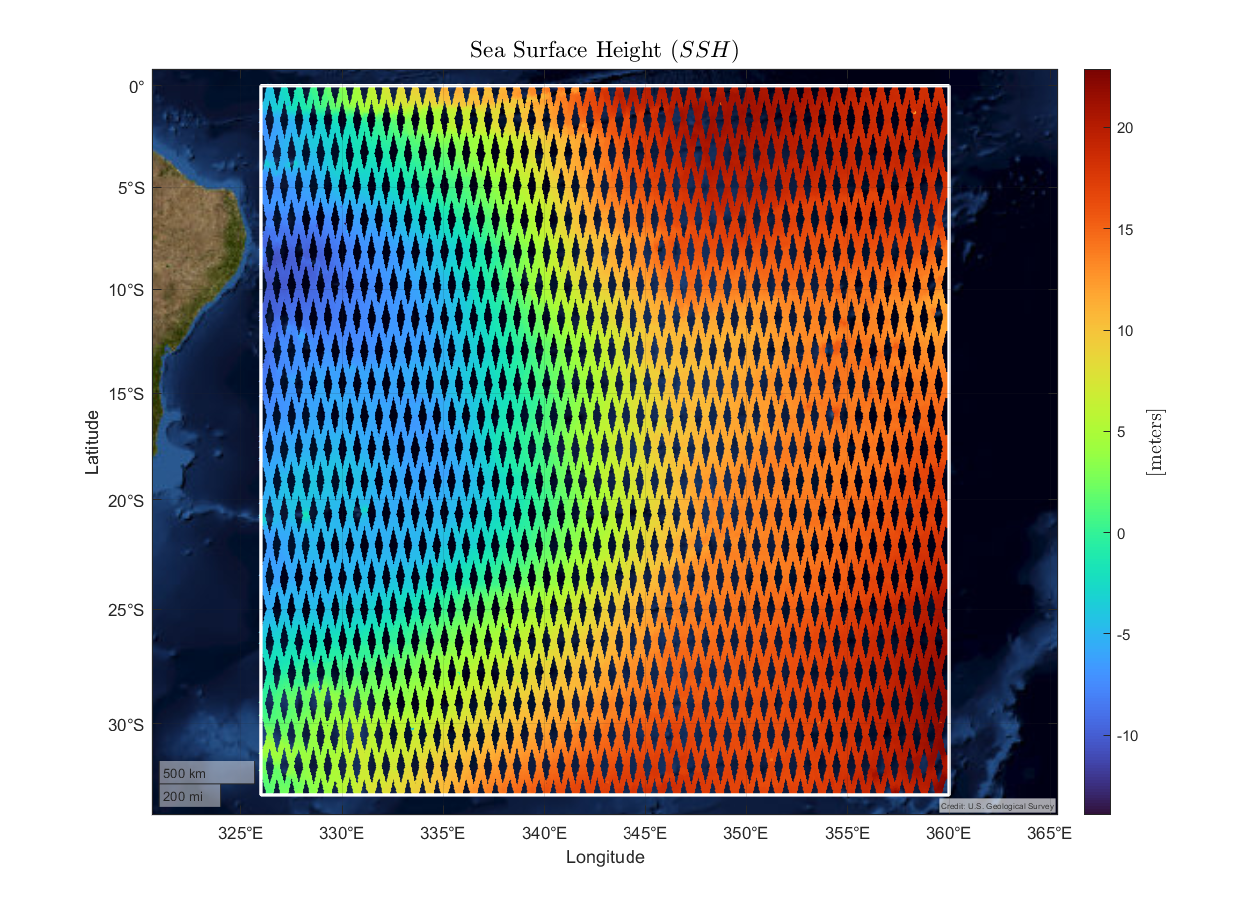
\includegraphics[height=7.5cm]{../Plots/SSH.pdf}
		\caption{SSH values during the specified time period.}
		\label{fig:SSH}
	\end{figure}
	\clearpage
	
	\section{Geoid Height Calculation}
	To calculate the geoid height according to Equation \ref{eq:relation}, a grid with $0.25^\circ$ intervals was defined within this area. The DOT and SSH values were interpolated at these points, and by calculating their difference, the geoid height was obtained. The interpolation results can be seen in Figures \ref{fig:DOTint} and \ref{fig:SSHint}. The calculated geoid height is also shown in Figure \ref{fig:N}.
	
	\begin{figure}[h!]
		\centering
		\includegraphics[width=16cm]{../Plots/InterpolatedDOT.pdf}
		\caption{Interpolated DOT values on the specified grid.}
		\label{fig:DOTint}
	\end{figure}
	
	\begin{figure}[h!]
		\centering
		\includegraphics[width=16cm]{../Plots/InterpolatedSSH.pdf}
		\caption{Interpolated SSH values on the specified grid.}
		\label{fig:SSHint}
	\end{figure}
	\clearpage
	
	\begin{figure}[h!]
		\centering
		\includegraphics[width=16cm]{../Plots/N.pdf}
		\caption{Calculated geoid height values on the specified grid.}
		\label{fig:N}
	\end{figure}
	
	\section{Gravity Anomaly Calculation}
	
	To calculate the gravity anomaly, the Inverse Stokes Formula (ISF) is used, which is expressed according to Equation \ref{eq:ISF}.
	
	\begin{equation}
		\Delta g_p(\varphi_p, \lambda_p) = - \frac{\bar{\gamma}}{R} N_p 
		- \frac{\bar{\gamma}}{16 \pi R} \iint_\sigma \frac{N_q - N_p}{\sin^3 \left(\frac{\psi}{2}\right)} 
		\label{eq:ISF}		
	\end{equation}
	
	In this Equation, $\lambda_p$ and $\varphi_p$ are the longitude and latitude of the points where the gravity anomaly is to be calculated. $\gamma$ is the average Earth gravity, which is considered as $980,665 mGal$, and $R$ is the mean radius of the Earth. $N_p$ and $N_q$ are, respectively, the geoid height of the point of interest and the geoid heights of the points within the integration area. $\sin^3 \left(\frac{\psi}{2}\right)$ can be calculated using Equation \ref{eq:sin}.

	\begin{equation}
		\sin^3\left(\frac{\psi}{2}\right) = \left[\sin^2\left(\frac{\varphi_p - \varphi_q}{2}\right) + \sin^2\left(\frac{\lambda_p - \lambda_q}{2}\right) \cos(\varphi_p)\cos(\varphi_q)\right]^{\frac{3}{2}}
		\label{eq:sin}
	\end{equation}

	The discrete form of the Inverse Stokes Formula used in this project is given by Equation \ref{eq:ISF_dis}.
	
	\begin{equation}
		\Delta g_p(\varphi_p, \lambda_p) = 
		- \frac{\overline{\gamma}}{R} N_p 
		- \frac{\Delta \varphi \Delta \lambda}{16 \pi R} \overline{\gamma}
		\sum_{\varphi_q = \varphi_1}^{\varphi_n} 
		\sum_{\lambda_q = \lambda_1}^{\lambda_n} 
		\frac{(N_q - N_p) \cos(\varphi_q)}
		{\sin^3 \left( \frac{\psi}{2} \right)}
		\label{eq:ISF_dis}
	\end{equation}
	
	$\Delta \lambda$ and $\Delta \varphi$ are the grid spacing in the longitude and latitude directions, respectively. The results obtained and the calculated gravity anomaly are shown in Figure \ref{fig:dg}. For validation purposes, the XGM2019 model was also used, and the gravity anomaly from this model is shown in Figure \ref{fig:XGM2019}. 
	
	\clearpage
	
	\begin{figure}[h!]
		\centering
		\includegraphics[width=16cm]{../Plots/dg.pdf}
		\caption{Calculated gravity anomaly values on the specified grid.}
		\label{fig:dg}
	\end{figure}
	
	
	\begin{figure}[h!]
		\centering
		\includegraphics[width=16cm]{../Plots/XGM2019dg.pdf}
		\caption{Gravity anomaly values obtained from the XGM2019 model.}
		\label{fig:XGM2019}
	\end{figure}
	
\end{document}


